\begin{figure}[ht]
\centering

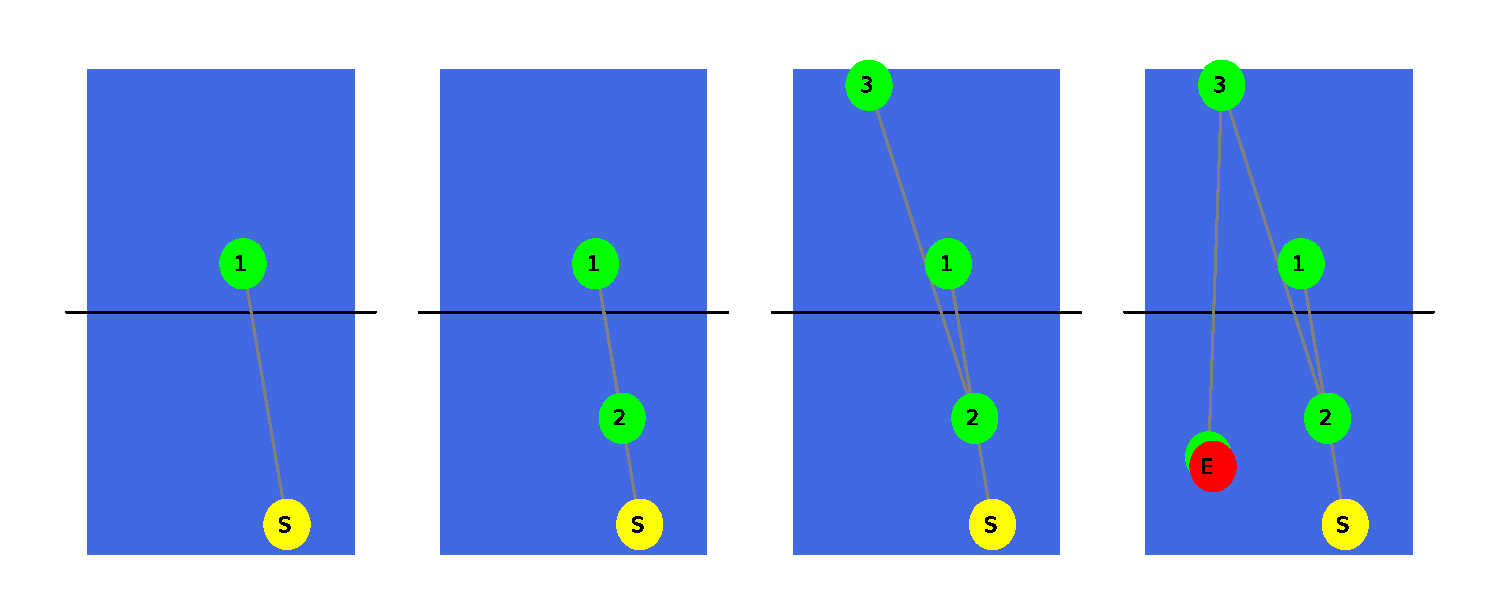
\includegraphics[width=8.5cm]{plots/chiang1.pdf}
\caption{Progression of a rally demonstrating the landing point of each ball bounce. Yellow indicates service which starts a rally and red indicates an error ending the rally. Green indicates all other ball bounces. Based on data from OSAI  \cite{OSAI}.}
%\denes{Please remove all margins on these plots}}

\label{fig:sequence}
\end{figure}

\begin{figure}[ht]
\centering

%\vspace{-2em}
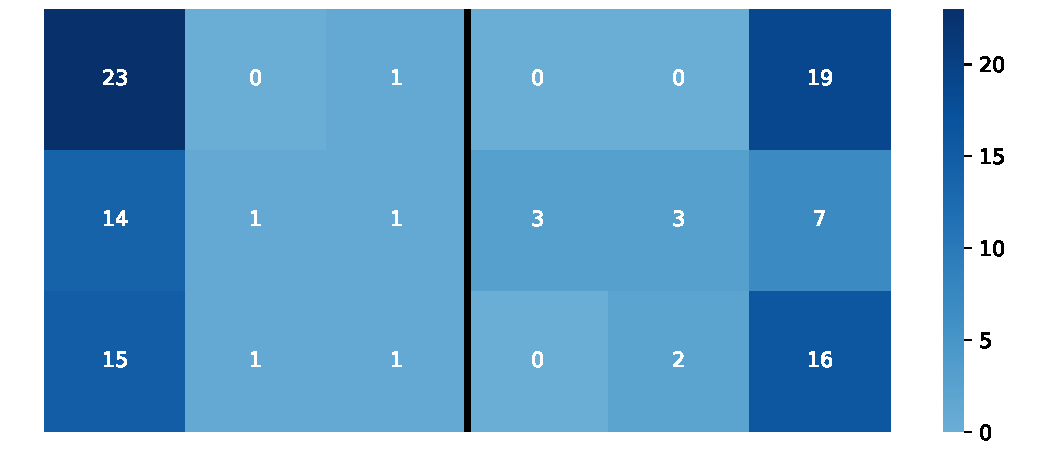
\includegraphics[width=8cm]{plots/chiang2.pdf}
\caption{Location of the last bounce of the winning ball, summed over an example match. Each side of the table is split into nine equal parts.}

\label{fig:pos}
\end{figure}


\begin{figure}[t]
\centering
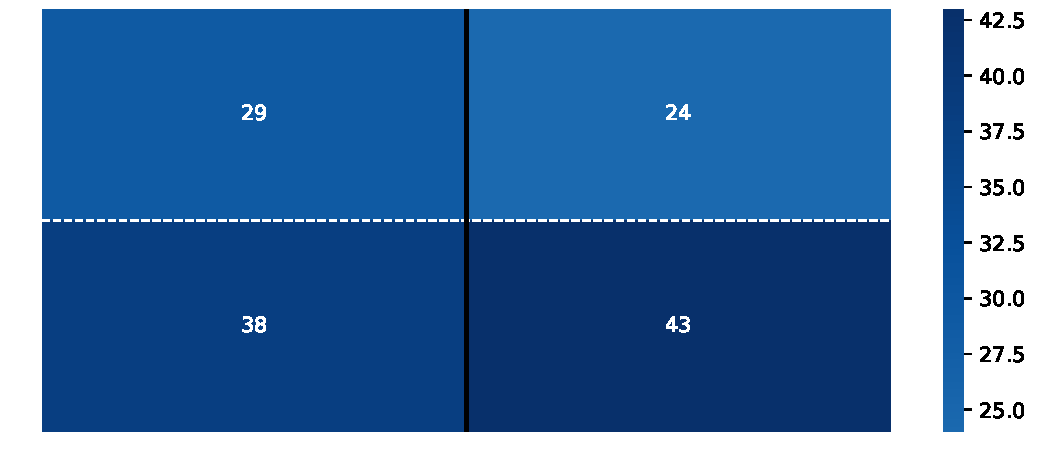
\includegraphics[width=8cm]{plots/chiang3a.pdf}
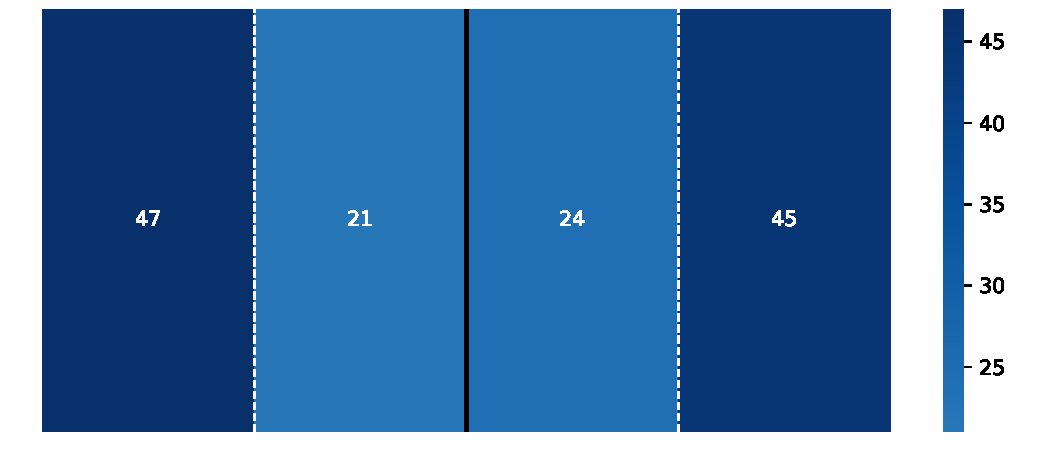
\includegraphics[width=8cm]{plots/chiang3b.pdf}
\caption{Number of points won by forehand vs. backhand (top);  by a short vs. long rally (bottom) in an example match \cite{OSAI}.}

\label{fig:svlr}
\end{figure}

\section{Dataset} \label{sec:dataset}
Our primary source of data are automatic captures from TTNet \cite{voeikov2020ttnet}, released by OSAI \cite{OSAI}. We use Tokyo 2020 Olympics and Tischtennis-Bundesliga (German table tennis league) data, which include men and women's singles matches. Potential features include player  rank and in-match statistics such as percentage of points won on serve and receive, stroke  and error types. Match progression can be plotted for each set, recording the location of each ball bounce (see \figref{sequence}).

%Interactive maps that demonstrated the ball position of each shot on the table, as well as the stroke type were also accessible. The progression of a rally and location of each ball bounce can be mapped into a sequence (see \figref{sequence}).

To reduce the dimensionality of the problem, a rally can be represented as the location of the winning shot. Furthermore, each half of the table can be split into nine equal sections, and the location of winning shots can be grouped (\figref{pos}). Further grouping can involve the number of forehands and the number of backhands used to win a point, or whether it was a `short' or `long' rally (\figref{svlr}). % The use of these features is discussed in  \secref{features}.
%\denes{which version? Fig 3 or 4?}.
Samples with missing data entries were removed from the dataset.

 
 %One of the main challenges in constructing a successful result predictor is the selection of salient features. To address this, we carefully hand picked features that we thought would be the most influential in a match based on existing domain knowledge on the problem.